\documentclass[twoside]{book}

% Packages required by doxygen
\usepackage{fixltx2e}
\usepackage{calc}
\usepackage{doxygen}
\usepackage[export]{adjustbox} % also loads graphicx
\usepackage{graphicx}
\usepackage[utf8]{inputenc}
\usepackage{makeidx}
\usepackage{multicol}
\usepackage{multirow}
\PassOptionsToPackage{warn}{textcomp}
\usepackage{textcomp}
\usepackage[nointegrals]{wasysym}
\usepackage[table]{xcolor}

% Font selection
\usepackage[T1]{fontenc}
\usepackage[scaled=.90]{helvet}
\usepackage{courier}
\usepackage{amssymb}
\usepackage{sectsty}
\renewcommand{\familydefault}{\sfdefault}
\allsectionsfont{%
  \fontseries{bc}\selectfont%
  \color{darkgray}%
}
\renewcommand{\DoxyLabelFont}{%
  \fontseries{bc}\selectfont%
  \color{darkgray}%
}
\newcommand{\+}{\discretionary{\mbox{\scriptsize$\hookleftarrow$}}{}{}}

% Page & text layout
\usepackage{geometry}
\geometry{%
  a4paper,%
  top=2.5cm,%
  bottom=2.5cm,%
  left=2.5cm,%
  right=2.5cm%
}
\tolerance=750
\hfuzz=15pt
\hbadness=750
\setlength{\emergencystretch}{15pt}
\setlength{\parindent}{0cm}
\setlength{\parskip}{0.2cm}
\makeatletter
\renewcommand{\paragraph}{%
  \@startsection{paragraph}{4}{0ex}{-1.0ex}{1.0ex}{%
    \normalfont\normalsize\bfseries\SS@parafont%
  }%
}
\renewcommand{\subparagraph}{%
  \@startsection{subparagraph}{5}{0ex}{-1.0ex}{1.0ex}{%
    \normalfont\normalsize\bfseries\SS@subparafont%
  }%
}
\makeatother

% Headers & footers
\usepackage{fancyhdr}
\pagestyle{fancyplain}
\fancyhead[LE]{\fancyplain{}{\bfseries\thepage}}
\fancyhead[CE]{\fancyplain{}{}}
\fancyhead[RE]{\fancyplain{}{\bfseries\leftmark}}
\fancyhead[LO]{\fancyplain{}{\bfseries\rightmark}}
\fancyhead[CO]{\fancyplain{}{}}
\fancyhead[RO]{\fancyplain{}{\bfseries\thepage}}
\fancyfoot[LE]{\fancyplain{}{}}
\fancyfoot[CE]{\fancyplain{}{}}
\fancyfoot[RE]{\fancyplain{}{\bfseries\scriptsize Generated on Fri Jul 10 2015 12\+:10\+:55 for Ueb11 by Doxygen }}
\fancyfoot[LO]{\fancyplain{}{\bfseries\scriptsize Generated on Fri Jul 10 2015 12\+:10\+:55 for Ueb11 by Doxygen }}
\fancyfoot[CO]{\fancyplain{}{}}
\fancyfoot[RO]{\fancyplain{}{}}
\renewcommand{\footrulewidth}{0.4pt}
\renewcommand{\chaptermark}[1]{%
  \markboth{#1}{}%
}
\renewcommand{\sectionmark}[1]{%
  \markright{\thesection\ #1}%
}

% Indices & bibliography
\usepackage{natbib}
\usepackage[titles]{tocloft}
\setcounter{tocdepth}{3}
\setcounter{secnumdepth}{5}
\makeindex

% Hyperlinks (required, but should be loaded last)
\usepackage{ifpdf}
\ifpdf
  \usepackage[pdftex,pagebackref=true]{hyperref}
\else
  \usepackage[ps2pdf,pagebackref=true]{hyperref}
\fi
\hypersetup{%
  colorlinks=true,%
  linkcolor=blue,%
  citecolor=blue,%
  unicode%
}

% Custom commands
\newcommand{\clearemptydoublepage}{%
  \newpage{\pagestyle{empty}\cleardoublepage}%
}


%===== C O N T E N T S =====

\begin{document}

% Titlepage & ToC
\hypersetup{pageanchor=false,
             bookmarks=true,
             bookmarksnumbered=true,
             pdfencoding=unicode
            }
\pagenumbering{roman}
\begin{titlepage}
\vspace*{7cm}
\begin{center}%
{\Large Ueb11 }\\
\vspace*{1cm}
{\large Generated by Doxygen 1.8.9.1}\\
\vspace*{0.5cm}
{\small Fri Jul 10 2015 12:10:55}\\
\end{center}
\end{titlepage}
\clearemptydoublepage
\tableofcontents
\clearemptydoublepage
\pagenumbering{arabic}
\hypersetup{pageanchor=true}

%--- Begin generated contents ---
\chapter{Hierarchical Index}
\section{Class Hierarchy}
This inheritance list is sorted roughly, but not completely, alphabetically\+:\begin{DoxyCompactList}
\item \contentsline{section}{Projektbestandteil}{\pageref{classProjektbestandteil}}{}
\begin{DoxyCompactList}
\item \contentsline{section}{Aufgabe}{\pageref{classAufgabe}}{}
\item \contentsline{section}{Produkt}{\pageref{classProdukt}}{}
\item \contentsline{section}{Projekt}{\pageref{classProjekt}}{}
\end{DoxyCompactList}
\end{DoxyCompactList}

\chapter{Class Index}
\section{Class List}
Here are the classes, structs, unions and interfaces with brief descriptions\+:\begin{DoxyCompactList}
\item\contentsline{section}{\hyperlink{classAufgabe}{Aufgabe} }{\pageref{classAufgabe}}{}
\item\contentsline{section}{\hyperlink{classProdukt}{Produkt} }{\pageref{classProdukt}}{}
\item\contentsline{section}{\hyperlink{classProjekt}{Projekt} }{\pageref{classProjekt}}{}
\item\contentsline{section}{\hyperlink{classProjektbestandteil}{Projektbestandteil} }{\pageref{classProjektbestandteil}}{}
\end{DoxyCompactList}

\chapter{File Index}
\section{File List}
Here is a list of all files with brief descriptions\+:\begin{DoxyCompactList}
\item\contentsline{section}{\hyperlink{Aufgabe_8cpp}{Aufgabe.\+cpp} }{\pageref{Aufgabe_8cpp}}{}
\item\contentsline{section}{\hyperlink{Aufgabe_8h}{Aufgabe.\+h} }{\pageref{Aufgabe_8h}}{}
\item\contentsline{section}{\hyperlink{Produkt_8cpp}{Produkt.\+cpp} }{\pageref{Produkt_8cpp}}{}
\item\contentsline{section}{\hyperlink{Produkt_8h}{Produkt.\+h} }{\pageref{Produkt_8h}}{}
\item\contentsline{section}{\hyperlink{Projekt_8cpp}{Projekt.\+cpp} }{\pageref{Projekt_8cpp}}{}
\item\contentsline{section}{\hyperlink{Projekt_8h}{Projekt.\+h} }{\pageref{Projekt_8h}}{}
\item\contentsline{section}{\hyperlink{Projektbestandteil_8cpp}{Projektbestandteil.\+cpp} }{\pageref{Projektbestandteil_8cpp}}{}
\item\contentsline{section}{\hyperlink{Projektbestandteil_8h}{Projektbestandteil.\+h} }{\pageref{Projektbestandteil_8h}}{}
\item\contentsline{section}{\hyperlink{ueb11_8cpp}{ueb11.\+cpp} }{\pageref{ueb11_8cpp}}{}
\end{DoxyCompactList}

\chapter{Class Documentation}
\hypertarget{classAufgabe}{}\section{Aufgabe Class Reference}
\label{classAufgabe}\index{Aufgabe@{Aufgabe}}


{\ttfamily \#include $<$Aufgabe.\+h$>$}

Inheritance diagram for Aufgabe\+:\begin{figure}[H]
\begin{center}
\leavevmode
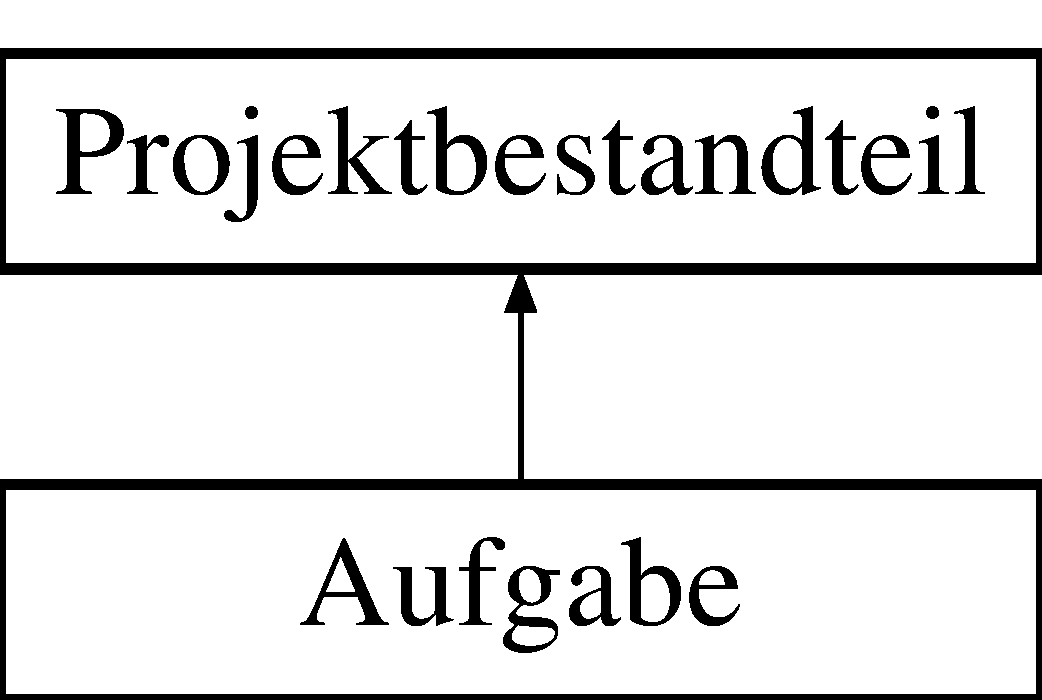
\includegraphics[height=2.000000cm]{classAufgabe}
\end{center}
\end{figure}
\subsection*{Public Member Functions}
\begin{DoxyCompactItemize}
\item 
\hyperlink{classAufgabe_a27e05f3a06ff3120e85225e3685bd8b7}{Aufgabe} (string \hyperlink{classProjektbestandteil_a3592f75d5870371bd87c9a057f31241e}{name}, string \hyperlink{classProjektbestandteil_a68c5cc53ee0c402c82e333493f460ecb}{beschreibung}, int \hyperlink{classAufgabe_a5600f7219bcc8e1f048a303873edc14b}{aufwand})
\item 
virtual \hyperlink{classAufgabe_a432c555be1087f0dcdf21a39688eb22d}{$\sim$\+Aufgabe} ()
\item 
virtual double \hyperlink{classAufgabe_abae0fc05c5038ef24db303ec6223758f}{berechne\+Kosten} (double stundensatz)
\end{DoxyCompactItemize}
\subsection*{Private Attributes}
\begin{DoxyCompactItemize}
\item 
int \hyperlink{classAufgabe_a5600f7219bcc8e1f048a303873edc14b}{aufwand}
\end{DoxyCompactItemize}


\subsection{Constructor \& Destructor Documentation}
\hypertarget{classAufgabe_a27e05f3a06ff3120e85225e3685bd8b7}{}\index{Aufgabe@{Aufgabe}!Aufgabe@{Aufgabe}}
\index{Aufgabe@{Aufgabe}!Aufgabe@{Aufgabe}}
\subsubsection[{Aufgabe(string name, string beschreibung, int aufwand)}]{\setlength{\rightskip}{0pt plus 5cm}Aufgabe\+::\+Aufgabe (
\begin{DoxyParamCaption}
\item[{string}]{name, }
\item[{string}]{beschreibung, }
\item[{int}]{aufwand}
\end{DoxyParamCaption}
)}\label{classAufgabe_a27e05f3a06ff3120e85225e3685bd8b7}
\hypertarget{classAufgabe_a432c555be1087f0dcdf21a39688eb22d}{}\index{Aufgabe@{Aufgabe}!````~Aufgabe@{$\sim$\+Aufgabe}}
\index{````~Aufgabe@{$\sim$\+Aufgabe}!Aufgabe@{Aufgabe}}
\subsubsection[{$\sim$\+Aufgabe()}]{\setlength{\rightskip}{0pt plus 5cm}Aufgabe\+::$\sim$\+Aufgabe (
\begin{DoxyParamCaption}
{}
\end{DoxyParamCaption}
)\hspace{0.3cm}{\ttfamily [virtual]}}\label{classAufgabe_a432c555be1087f0dcdf21a39688eb22d}


\subsection{Member Function Documentation}
\hypertarget{classAufgabe_abae0fc05c5038ef24db303ec6223758f}{}\index{Aufgabe@{Aufgabe}!berechne\+Kosten@{berechne\+Kosten}}
\index{berechne\+Kosten@{berechne\+Kosten}!Aufgabe@{Aufgabe}}
\subsubsection[{berechne\+Kosten(double stundensatz)}]{\setlength{\rightskip}{0pt plus 5cm}double Aufgabe\+::berechne\+Kosten (
\begin{DoxyParamCaption}
\item[{double}]{stundensatz}
\end{DoxyParamCaption}
)\hspace{0.3cm}{\ttfamily [virtual]}}\label{classAufgabe_abae0fc05c5038ef24db303ec6223758f}


Implements \hyperlink{classProjektbestandteil_acfbc3a13db3a04de51ec9578436b4736}{Projektbestandteil}.



\subsection{Member Data Documentation}
\hypertarget{classAufgabe_a5600f7219bcc8e1f048a303873edc14b}{}\index{Aufgabe@{Aufgabe}!aufwand@{aufwand}}
\index{aufwand@{aufwand}!Aufgabe@{Aufgabe}}
\subsubsection[{aufwand}]{\setlength{\rightskip}{0pt plus 5cm}int Aufgabe\+::aufwand\hspace{0.3cm}{\ttfamily [private]}}\label{classAufgabe_a5600f7219bcc8e1f048a303873edc14b}


The documentation for this class was generated from the following files\+:\begin{DoxyCompactItemize}
\item 
\hyperlink{Aufgabe_8h}{Aufgabe.\+h}\item 
\hyperlink{Aufgabe_8cpp}{Aufgabe.\+cpp}\end{DoxyCompactItemize}

\hypertarget{classProdukt}{}\section{Produkt Class Reference}
\label{classProdukt}\index{Produkt@{Produkt}}


{\ttfamily \#include $<$Produkt.\+h$>$}

Inheritance diagram for Produkt\+:\begin{figure}[H]
\begin{center}
\leavevmode
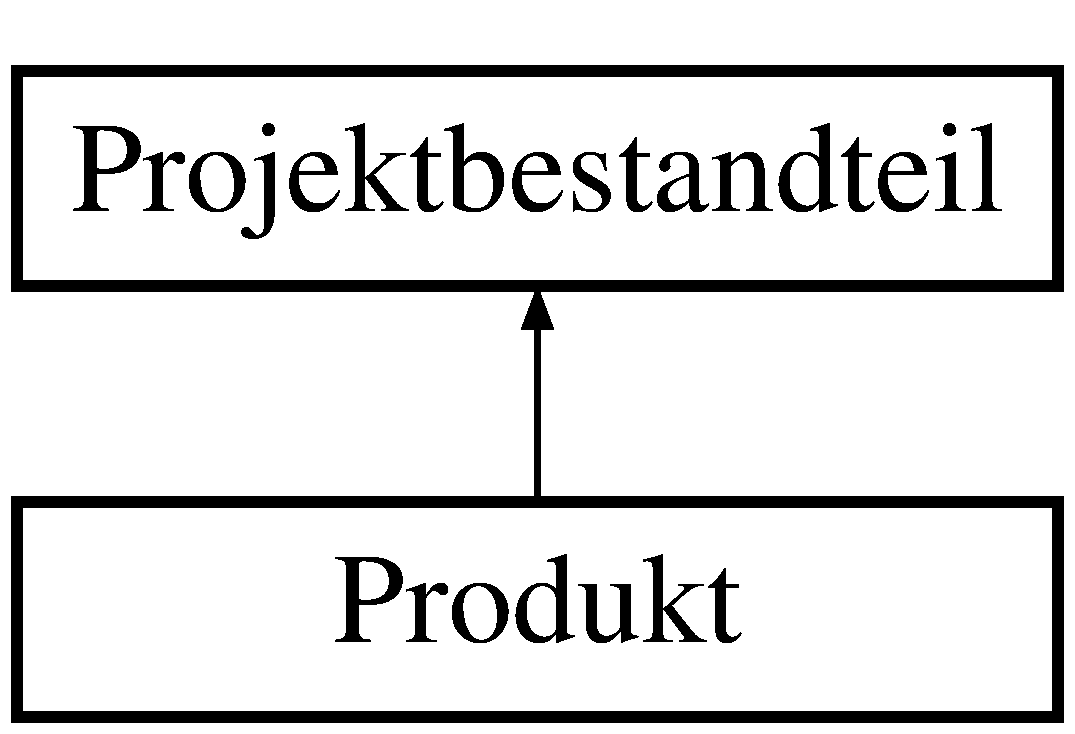
\includegraphics[height=2.000000cm]{classProdukt}
\end{center}
\end{figure}
\subsection*{Public Member Functions}
\begin{DoxyCompactItemize}
\item 
\hyperlink{classProdukt_a9baacb2e08b3cc4a7dd951810702bd67}{Produkt} (string \hyperlink{classProjektbestandteil_a3592f75d5870371bd87c9a057f31241e}{name}, string \hyperlink{classProjektbestandteil_a68c5cc53ee0c402c82e333493f460ecb}{beschreibung}, double \hyperlink{classProdukt_ad7901109c0a1ec4ac65fd898d6d8405b}{produktionskosten})
\item 
virtual \hyperlink{classProdukt_aa73d71caf7d4e9c8590f726faf263290}{$\sim$\+Produkt} ()
\item 
virtual double \hyperlink{classProdukt_aec53e84c49b971d78cf4b7881afc8c20}{berechne\+Kosten} (double stunden\+Satz)
\end{DoxyCompactItemize}
\subsection*{Private Attributes}
\begin{DoxyCompactItemize}
\item 
double \hyperlink{classProdukt_ad7901109c0a1ec4ac65fd898d6d8405b}{produktionskosten}
\end{DoxyCompactItemize}


\subsection{Constructor \& Destructor Documentation}
\hypertarget{classProdukt_a9baacb2e08b3cc4a7dd951810702bd67}{}\index{Produkt@{Produkt}!Produkt@{Produkt}}
\index{Produkt@{Produkt}!Produkt@{Produkt}}
\subsubsection[{Produkt(string name, string beschreibung, double produktionskosten)}]{\setlength{\rightskip}{0pt plus 5cm}Produkt\+::\+Produkt (
\begin{DoxyParamCaption}
\item[{string}]{name, }
\item[{string}]{beschreibung, }
\item[{double}]{produktionskosten}
\end{DoxyParamCaption}
)}\label{classProdukt_a9baacb2e08b3cc4a7dd951810702bd67}
\hypertarget{classProdukt_aa73d71caf7d4e9c8590f726faf263290}{}\index{Produkt@{Produkt}!````~Produkt@{$\sim$\+Produkt}}
\index{````~Produkt@{$\sim$\+Produkt}!Produkt@{Produkt}}
\subsubsection[{$\sim$\+Produkt()}]{\setlength{\rightskip}{0pt plus 5cm}Produkt\+::$\sim$\+Produkt (
\begin{DoxyParamCaption}
{}
\end{DoxyParamCaption}
)\hspace{0.3cm}{\ttfamily [virtual]}}\label{classProdukt_aa73d71caf7d4e9c8590f726faf263290}


\subsection{Member Function Documentation}
\hypertarget{classProdukt_aec53e84c49b971d78cf4b7881afc8c20}{}\index{Produkt@{Produkt}!berechne\+Kosten@{berechne\+Kosten}}
\index{berechne\+Kosten@{berechne\+Kosten}!Produkt@{Produkt}}
\subsubsection[{berechne\+Kosten(double stunden\+Satz)}]{\setlength{\rightskip}{0pt plus 5cm}double Produkt\+::berechne\+Kosten (
\begin{DoxyParamCaption}
\item[{double}]{stunden\+Satz}
\end{DoxyParamCaption}
)\hspace{0.3cm}{\ttfamily [virtual]}}\label{classProdukt_aec53e84c49b971d78cf4b7881afc8c20}


Implements \hyperlink{classProjektbestandteil_acfbc3a13db3a04de51ec9578436b4736}{Projektbestandteil}.



\subsection{Member Data Documentation}
\hypertarget{classProdukt_ad7901109c0a1ec4ac65fd898d6d8405b}{}\index{Produkt@{Produkt}!produktionskosten@{produktionskosten}}
\index{produktionskosten@{produktionskosten}!Produkt@{Produkt}}
\subsubsection[{produktionskosten}]{\setlength{\rightskip}{0pt plus 5cm}double Produkt\+::produktionskosten\hspace{0.3cm}{\ttfamily [private]}}\label{classProdukt_ad7901109c0a1ec4ac65fd898d6d8405b}


The documentation for this class was generated from the following files\+:\begin{DoxyCompactItemize}
\item 
\hyperlink{Produkt_8h}{Produkt.\+h}\item 
\hyperlink{Produkt_8cpp}{Produkt.\+cpp}\end{DoxyCompactItemize}

\hypertarget{classProjekt}{}\section{Projekt Class Reference}
\label{classProjekt}\index{Projekt@{Projekt}}


{\ttfamily \#include $<$Projekt.\+h$>$}

Inheritance diagram for Projekt\+:\begin{figure}[H]
\begin{center}
\leavevmode
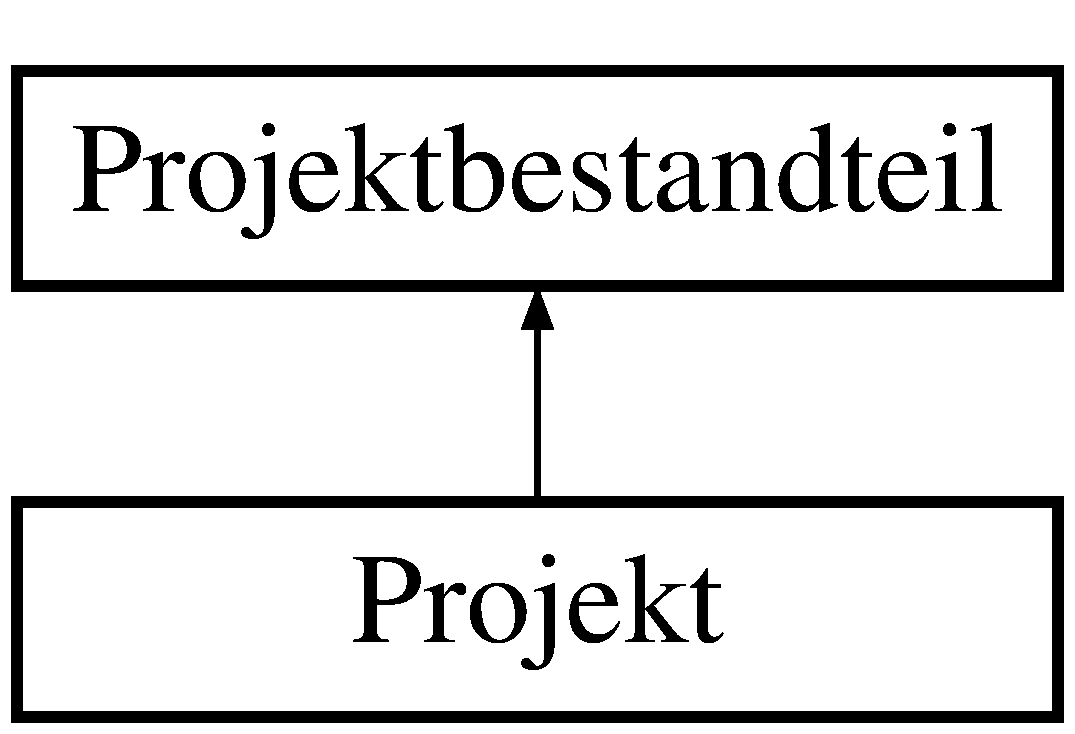
\includegraphics[height=2.000000cm]{classProjekt}
\end{center}
\end{figure}
\subsection*{Public Member Functions}
\begin{DoxyCompactItemize}
\item 
\hyperlink{classProjekt_add70b5b0cdf0352c035894b25a138613}{Projekt} (string \hyperlink{classProjektbestandteil_a3592f75d5870371bd87c9a057f31241e}{name}, string Beschreibung, double \hyperlink{classProjekt_afac3a0828a5f2e976af1dbb46ac712ca}{stunden\+Satz})
\item 
virtual \hyperlink{classProjekt_a309c58dde12f9ae62764ad7a0f99056f}{$\sim$\+Projekt} ()
\item 
void \hyperlink{classProjekt_a6980c205cb2597e8f8af453d2902894a}{add} (\hyperlink{classProjektbestandteil}{Projektbestandteil} $\ast$projekbestandteil)
\item 
void \hyperlink{classProjekt_a21497c043d324409785f5dec182e39a1}{remove} (string \hyperlink{classProjektbestandteil_a3592f75d5870371bd87c9a057f31241e}{name})
\item 
virtual double \hyperlink{classProjekt_ae26b381f70891f93fd28cec57565d784}{berechne\+Kosten} (double \hyperlink{classProjekt_afac3a0828a5f2e976af1dbb46ac712ca}{stunden\+Satz})
\end{DoxyCompactItemize}
\subsection*{Static Public Attributes}
\begin{DoxyCompactItemize}
\item 
static const int \hyperlink{classProjekt_a2828c8ece2df6372db85967f774e61a4}{max\+Parts} = 20
\end{DoxyCompactItemize}
\subsection*{Private Member Functions}
\begin{DoxyCompactItemize}
\item 
\hyperlink{classProjektbestandteil}{Projektbestandteil} $\ast$ \hyperlink{classProjekt_a3f180dc9888680454c5fce561945045f}{find\+Project\+Part} (string \hyperlink{classProjektbestandteil_a3592f75d5870371bd87c9a057f31241e}{name})
\item 
void \hyperlink{classProjekt_a9ae5e39c9b41223d6981c9ca5924922e}{delete\+All\+Parts} ()
\end{DoxyCompactItemize}
\subsection*{Private Attributes}
\begin{DoxyCompactItemize}
\item 
\hyperlink{classProjektbestandteil}{Projektbestandteil} $\ast$$\ast$ \hyperlink{classProjekt_a14ba023886dcaffaddbebb7623b0067b}{teil\+Tab}
\item 
double \hyperlink{classProjekt_afac3a0828a5f2e976af1dbb46ac712ca}{stunden\+Satz}
\item 
int \hyperlink{classProjekt_ac705642faf893d995f60f617183f0ed7}{teile}
\end{DoxyCompactItemize}


\subsection{Constructor \& Destructor Documentation}
\hypertarget{classProjekt_add70b5b0cdf0352c035894b25a138613}{}\index{Projekt@{Projekt}!Projekt@{Projekt}}
\index{Projekt@{Projekt}!Projekt@{Projekt}}
\subsubsection[{Projekt(string name, string Beschreibung, double stunden\+Satz)}]{\setlength{\rightskip}{0pt plus 5cm}Projekt\+::\+Projekt (
\begin{DoxyParamCaption}
\item[{string}]{name, }
\item[{string}]{Beschreibung, }
\item[{double}]{stunden\+Satz}
\end{DoxyParamCaption}
)}\label{classProjekt_add70b5b0cdf0352c035894b25a138613}
\hypertarget{classProjekt_a309c58dde12f9ae62764ad7a0f99056f}{}\index{Projekt@{Projekt}!````~Projekt@{$\sim$\+Projekt}}
\index{````~Projekt@{$\sim$\+Projekt}!Projekt@{Projekt}}
\subsubsection[{$\sim$\+Projekt()}]{\setlength{\rightskip}{0pt plus 5cm}Projekt\+::$\sim$\+Projekt (
\begin{DoxyParamCaption}
{}
\end{DoxyParamCaption}
)\hspace{0.3cm}{\ttfamily [virtual]}}\label{classProjekt_a309c58dde12f9ae62764ad7a0f99056f}


\subsection{Member Function Documentation}
\hypertarget{classProjekt_a6980c205cb2597e8f8af453d2902894a}{}\index{Projekt@{Projekt}!add@{add}}
\index{add@{add}!Projekt@{Projekt}}
\subsubsection[{add(\+Projektbestandteil $\ast$projekbestandteil)}]{\setlength{\rightskip}{0pt plus 5cm}void Projekt\+::add (
\begin{DoxyParamCaption}
\item[{{\bf Projektbestandteil} $\ast$}]{projekbestandteil}
\end{DoxyParamCaption}
)}\label{classProjekt_a6980c205cb2597e8f8af453d2902894a}
\hypertarget{classProjekt_ae26b381f70891f93fd28cec57565d784}{}\index{Projekt@{Projekt}!berechne\+Kosten@{berechne\+Kosten}}
\index{berechne\+Kosten@{berechne\+Kosten}!Projekt@{Projekt}}
\subsubsection[{berechne\+Kosten(double stunden\+Satz)}]{\setlength{\rightskip}{0pt plus 5cm}double Projekt\+::berechne\+Kosten (
\begin{DoxyParamCaption}
\item[{double}]{stunden\+Satz}
\end{DoxyParamCaption}
)\hspace{0.3cm}{\ttfamily [virtual]}}\label{classProjekt_ae26b381f70891f93fd28cec57565d784}


Implements \hyperlink{classProjektbestandteil_acfbc3a13db3a04de51ec9578436b4736}{Projektbestandteil}.

\hypertarget{classProjekt_a9ae5e39c9b41223d6981c9ca5924922e}{}\index{Projekt@{Projekt}!delete\+All\+Parts@{delete\+All\+Parts}}
\index{delete\+All\+Parts@{delete\+All\+Parts}!Projekt@{Projekt}}
\subsubsection[{delete\+All\+Parts()}]{\setlength{\rightskip}{0pt plus 5cm}void Projekt\+::delete\+All\+Parts (
\begin{DoxyParamCaption}
{}
\end{DoxyParamCaption}
)\hspace{0.3cm}{\ttfamily [private]}}\label{classProjekt_a9ae5e39c9b41223d6981c9ca5924922e}
\hypertarget{classProjekt_a3f180dc9888680454c5fce561945045f}{}\index{Projekt@{Projekt}!find\+Project\+Part@{find\+Project\+Part}}
\index{find\+Project\+Part@{find\+Project\+Part}!Projekt@{Projekt}}
\subsubsection[{find\+Project\+Part(string name)}]{\setlength{\rightskip}{0pt plus 5cm}{\bf Projektbestandteil}$\ast$ Projekt\+::find\+Project\+Part (
\begin{DoxyParamCaption}
\item[{string}]{name}
\end{DoxyParamCaption}
)\hspace{0.3cm}{\ttfamily [private]}}\label{classProjekt_a3f180dc9888680454c5fce561945045f}
\hypertarget{classProjekt_a21497c043d324409785f5dec182e39a1}{}\index{Projekt@{Projekt}!remove@{remove}}
\index{remove@{remove}!Projekt@{Projekt}}
\subsubsection[{remove(string name)}]{\setlength{\rightskip}{0pt plus 5cm}void Projekt\+::remove (
\begin{DoxyParamCaption}
\item[{string}]{name}
\end{DoxyParamCaption}
)}\label{classProjekt_a21497c043d324409785f5dec182e39a1}


\subsection{Member Data Documentation}
\hypertarget{classProjekt_a2828c8ece2df6372db85967f774e61a4}{}\index{Projekt@{Projekt}!max\+Parts@{max\+Parts}}
\index{max\+Parts@{max\+Parts}!Projekt@{Projekt}}
\subsubsection[{max\+Parts}]{\setlength{\rightskip}{0pt plus 5cm}const int Projekt\+::max\+Parts = 20\hspace{0.3cm}{\ttfamily [static]}}\label{classProjekt_a2828c8ece2df6372db85967f774e61a4}
\hypertarget{classProjekt_afac3a0828a5f2e976af1dbb46ac712ca}{}\index{Projekt@{Projekt}!stunden\+Satz@{stunden\+Satz}}
\index{stunden\+Satz@{stunden\+Satz}!Projekt@{Projekt}}
\subsubsection[{stunden\+Satz}]{\setlength{\rightskip}{0pt plus 5cm}double Projekt\+::stunden\+Satz\hspace{0.3cm}{\ttfamily [private]}}\label{classProjekt_afac3a0828a5f2e976af1dbb46ac712ca}
\hypertarget{classProjekt_ac705642faf893d995f60f617183f0ed7}{}\index{Projekt@{Projekt}!teile@{teile}}
\index{teile@{teile}!Projekt@{Projekt}}
\subsubsection[{teile}]{\setlength{\rightskip}{0pt plus 5cm}int Projekt\+::teile\hspace{0.3cm}{\ttfamily [private]}}\label{classProjekt_ac705642faf893d995f60f617183f0ed7}
\hypertarget{classProjekt_a14ba023886dcaffaddbebb7623b0067b}{}\index{Projekt@{Projekt}!teil\+Tab@{teil\+Tab}}
\index{teil\+Tab@{teil\+Tab}!Projekt@{Projekt}}
\subsubsection[{teil\+Tab}]{\setlength{\rightskip}{0pt plus 5cm}{\bf Projektbestandteil}$\ast$$\ast$ Projekt\+::teil\+Tab\hspace{0.3cm}{\ttfamily [private]}}\label{classProjekt_a14ba023886dcaffaddbebb7623b0067b}


The documentation for this class was generated from the following files\+:\begin{DoxyCompactItemize}
\item 
\hyperlink{Projekt_8h}{Projekt.\+h}\item 
\hyperlink{Projekt_8cpp}{Projekt.\+cpp}\end{DoxyCompactItemize}

\hypertarget{classProjektbestandteil}{}\section{Projektbestandteil Class Reference}
\label{classProjektbestandteil}\index{Projektbestandteil@{Projektbestandteil}}


{\ttfamily \#include $<$Projektbestandteil.\+h$>$}

Inheritance diagram for Projektbestandteil\+:\begin{figure}[H]
\begin{center}
\leavevmode
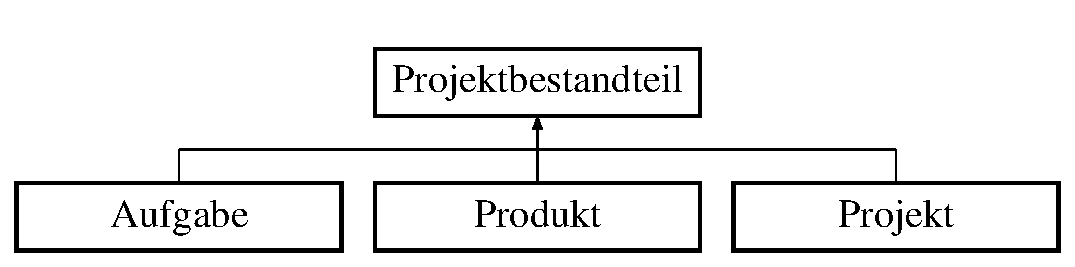
\includegraphics[height=2.000000cm]{classProjektbestandteil}
\end{center}
\end{figure}
\subsection*{Public Member Functions}
\begin{DoxyCompactItemize}
\item 
\hyperlink{classProjektbestandteil_ab7d77a751f69692590b5ad37445f1299}{Projektbestandteil} (string \hyperlink{classProjektbestandteil_a3592f75d5870371bd87c9a057f31241e}{name}, string \hyperlink{classProjektbestandteil_a68c5cc53ee0c402c82e333493f460ecb}{beschreibung})
\item 
virtual \hyperlink{classProjektbestandteil_a27f6a84885c2b783309403e5cf579ef1}{$\sim$\+Projektbestandteil} ()
\item 
const string \& \hyperlink{classProjektbestandteil_ac57329c90bc680e5bdc19bf8b66df5ed}{get\+Beschreibung} () const 
\item 
void \hyperlink{classProjektbestandteil_a317d5cd613fc5e62d2858d36f868de3b}{set\+Beschreibung} (const string \&\hyperlink{classProjektbestandteil_a68c5cc53ee0c402c82e333493f460ecb}{beschreibung})
\item 
const string \& \hyperlink{classProjektbestandteil_aeabecfd2533b8192fd07f596b2e426d0}{get\+Name} () const 
\item 
void \hyperlink{classProjektbestandteil_a9f11066ffbdcdad737a5cf2035392771}{set\+Name} (const string \&\hyperlink{classProjektbestandteil_a3592f75d5870371bd87c9a057f31241e}{name})
\item 
virtual double \hyperlink{classProjektbestandteil_acfbc3a13db3a04de51ec9578436b4736}{berechne\+Kosten} (double stunden\+Satz)=0
\end{DoxyCompactItemize}
\subsection*{Private Attributes}
\begin{DoxyCompactItemize}
\item 
string \hyperlink{classProjektbestandteil_a3592f75d5870371bd87c9a057f31241e}{name}
\item 
string \hyperlink{classProjektbestandteil_a68c5cc53ee0c402c82e333493f460ecb}{beschreibung}
\end{DoxyCompactItemize}


\subsection{Constructor \& Destructor Documentation}
\hypertarget{classProjektbestandteil_ab7d77a751f69692590b5ad37445f1299}{}\index{Projektbestandteil@{Projektbestandteil}!Projektbestandteil@{Projektbestandteil}}
\index{Projektbestandteil@{Projektbestandteil}!Projektbestandteil@{Projektbestandteil}}
\subsubsection[{Projektbestandteil(string name, string beschreibung)}]{\setlength{\rightskip}{0pt plus 5cm}Projektbestandteil\+::\+Projektbestandteil (
\begin{DoxyParamCaption}
\item[{string}]{name, }
\item[{string}]{beschreibung}
\end{DoxyParamCaption}
)\hspace{0.3cm}{\ttfamily [inline]}}\label{classProjektbestandteil_ab7d77a751f69692590b5ad37445f1299}
\hypertarget{classProjektbestandteil_a27f6a84885c2b783309403e5cf579ef1}{}\index{Projektbestandteil@{Projektbestandteil}!````~Projektbestandteil@{$\sim$\+Projektbestandteil}}
\index{````~Projektbestandteil@{$\sim$\+Projektbestandteil}!Projektbestandteil@{Projektbestandteil}}
\subsubsection[{$\sim$\+Projektbestandteil()}]{\setlength{\rightskip}{0pt plus 5cm}virtual Projektbestandteil\+::$\sim$\+Projektbestandteil (
\begin{DoxyParamCaption}
{}
\end{DoxyParamCaption}
)\hspace{0.3cm}{\ttfamily [inline]}, {\ttfamily [virtual]}}\label{classProjektbestandteil_a27f6a84885c2b783309403e5cf579ef1}


\subsection{Member Function Documentation}
\hypertarget{classProjektbestandteil_acfbc3a13db3a04de51ec9578436b4736}{}\index{Projektbestandteil@{Projektbestandteil}!berechne\+Kosten@{berechne\+Kosten}}
\index{berechne\+Kosten@{berechne\+Kosten}!Projektbestandteil@{Projektbestandteil}}
\subsubsection[{berechne\+Kosten(double stunden\+Satz)=0}]{\setlength{\rightskip}{0pt plus 5cm}virtual double Projektbestandteil\+::berechne\+Kosten (
\begin{DoxyParamCaption}
\item[{double}]{stunden\+Satz}
\end{DoxyParamCaption}
)\hspace{0.3cm}{\ttfamily [pure virtual]}}\label{classProjektbestandteil_acfbc3a13db3a04de51ec9578436b4736}


Implemented in \hyperlink{classProjekt_ae26b381f70891f93fd28cec57565d784}{Projekt}, \hyperlink{classAufgabe_abae0fc05c5038ef24db303ec6223758f}{Aufgabe}, and \hyperlink{classProdukt_aec53e84c49b971d78cf4b7881afc8c20}{Produkt}.

\hypertarget{classProjektbestandteil_ac57329c90bc680e5bdc19bf8b66df5ed}{}\index{Projektbestandteil@{Projektbestandteil}!get\+Beschreibung@{get\+Beschreibung}}
\index{get\+Beschreibung@{get\+Beschreibung}!Projektbestandteil@{Projektbestandteil}}
\subsubsection[{get\+Beschreibung() const }]{\setlength{\rightskip}{0pt plus 5cm}const string\& Projektbestandteil\+::get\+Beschreibung (
\begin{DoxyParamCaption}
{}
\end{DoxyParamCaption}
) const\hspace{0.3cm}{\ttfamily [inline]}}\label{classProjektbestandteil_ac57329c90bc680e5bdc19bf8b66df5ed}
\hypertarget{classProjektbestandteil_aeabecfd2533b8192fd07f596b2e426d0}{}\index{Projektbestandteil@{Projektbestandteil}!get\+Name@{get\+Name}}
\index{get\+Name@{get\+Name}!Projektbestandteil@{Projektbestandteil}}
\subsubsection[{get\+Name() const }]{\setlength{\rightskip}{0pt plus 5cm}const string\& Projektbestandteil\+::get\+Name (
\begin{DoxyParamCaption}
{}
\end{DoxyParamCaption}
) const\hspace{0.3cm}{\ttfamily [inline]}}\label{classProjektbestandteil_aeabecfd2533b8192fd07f596b2e426d0}
\hypertarget{classProjektbestandteil_a317d5cd613fc5e62d2858d36f868de3b}{}\index{Projektbestandteil@{Projektbestandteil}!set\+Beschreibung@{set\+Beschreibung}}
\index{set\+Beschreibung@{set\+Beschreibung}!Projektbestandteil@{Projektbestandteil}}
\subsubsection[{set\+Beschreibung(const string \&beschreibung)}]{\setlength{\rightskip}{0pt plus 5cm}void Projektbestandteil\+::set\+Beschreibung (
\begin{DoxyParamCaption}
\item[{const string \&}]{beschreibung}
\end{DoxyParamCaption}
)\hspace{0.3cm}{\ttfamily [inline]}}\label{classProjektbestandteil_a317d5cd613fc5e62d2858d36f868de3b}
\hypertarget{classProjektbestandteil_a9f11066ffbdcdad737a5cf2035392771}{}\index{Projektbestandteil@{Projektbestandteil}!set\+Name@{set\+Name}}
\index{set\+Name@{set\+Name}!Projektbestandteil@{Projektbestandteil}}
\subsubsection[{set\+Name(const string \&name)}]{\setlength{\rightskip}{0pt plus 5cm}void Projektbestandteil\+::set\+Name (
\begin{DoxyParamCaption}
\item[{const string \&}]{name}
\end{DoxyParamCaption}
)\hspace{0.3cm}{\ttfamily [inline]}}\label{classProjektbestandteil_a9f11066ffbdcdad737a5cf2035392771}


\subsection{Member Data Documentation}
\hypertarget{classProjektbestandteil_a68c5cc53ee0c402c82e333493f460ecb}{}\index{Projektbestandteil@{Projektbestandteil}!beschreibung@{beschreibung}}
\index{beschreibung@{beschreibung}!Projektbestandteil@{Projektbestandteil}}
\subsubsection[{beschreibung}]{\setlength{\rightskip}{0pt plus 5cm}string Projektbestandteil\+::beschreibung\hspace{0.3cm}{\ttfamily [private]}}\label{classProjektbestandteil_a68c5cc53ee0c402c82e333493f460ecb}
\hypertarget{classProjektbestandteil_a3592f75d5870371bd87c9a057f31241e}{}\index{Projektbestandteil@{Projektbestandteil}!name@{name}}
\index{name@{name}!Projektbestandteil@{Projektbestandteil}}
\subsubsection[{name}]{\setlength{\rightskip}{0pt plus 5cm}string Projektbestandteil\+::name\hspace{0.3cm}{\ttfamily [private]}}\label{classProjektbestandteil_a3592f75d5870371bd87c9a057f31241e}


The documentation for this class was generated from the following file\+:\begin{DoxyCompactItemize}
\item 
\hyperlink{Projektbestandteil_8h}{Projektbestandteil.\+h}\end{DoxyCompactItemize}

\chapter{File Documentation}
\hypertarget{Aufgabe_8cpp}{}\section{Aufgabe.\+cpp File Reference}
\label{Aufgabe_8cpp}\index{Aufgabe.\+cpp@{Aufgabe.\+cpp}}
{\ttfamily \#include \char`\"{}Aufgabe.\+h\char`\"{}}\\*

\hypertarget{Aufgabe_8h}{}\section{Aufgabe.\+h File Reference}
\label{Aufgabe_8h}\index{Aufgabe.\+h@{Aufgabe.\+h}}
{\ttfamily \#include \char`\"{}Projektbestandteil.\+h\char`\"{}}\\*
\subsection*{Classes}
\begin{DoxyCompactItemize}
\item 
class \hyperlink{classAufgabe}{Aufgabe}
\end{DoxyCompactItemize}

\hypertarget{Produkt_8cpp}{}\section{Produkt.\+cpp File Reference}
\label{Produkt_8cpp}\index{Produkt.\+cpp@{Produkt.\+cpp}}
{\ttfamily \#include \char`\"{}Produkt.\+h\char`\"{}}\\*

\hypertarget{Produkt_8h}{}\section{Produkt.\+h File Reference}
\label{Produkt_8h}\index{Produkt.\+h@{Produkt.\+h}}
{\ttfamily \#include \char`\"{}Projektbestandteil.\+h\char`\"{}}\\*
\subsection*{Classes}
\begin{DoxyCompactItemize}
\item 
class \hyperlink{classProdukt}{Produkt}
\end{DoxyCompactItemize}

\hypertarget{Projekt_8cpp}{}\section{Projekt.\+cpp File Reference}
\label{Projekt_8cpp}\index{Projekt.\+cpp@{Projekt.\+cpp}}
{\ttfamily \#include \char`\"{}Projekt.\+h\char`\"{}}\\*

\hypertarget{Projekt_8h}{}\section{Projekt.\+h File Reference}
\label{Projekt_8h}\index{Projekt.\+h@{Projekt.\+h}}
{\ttfamily \#include \char`\"{}Projektbestandteil.\+h\char`\"{}}\\*
\subsection*{Classes}
\begin{DoxyCompactItemize}
\item 
class \hyperlink{classProjekt}{Projekt}
\end{DoxyCompactItemize}

\hypertarget{Projektbestandteil_8cpp}{}\section{Projektbestandteil.\+cpp File Reference}
\label{Projektbestandteil_8cpp}\index{Projektbestandteil.\+cpp@{Projektbestandteil.\+cpp}}
{\ttfamily \#include \char`\"{}Projektbestandteil.\+h\char`\"{}}\\*

\hypertarget{Projektbestandteil_8h}{}\section{Projektbestandteil.\+h File Reference}
\label{Projektbestandteil_8h}\index{Projektbestandteil.\+h@{Projektbestandteil.\+h}}
{\ttfamily \#include $<$string$>$}\\*
\subsection*{Classes}
\begin{DoxyCompactItemize}
\item 
class \hyperlink{classProjektbestandteil}{Projektbestandteil}
\end{DoxyCompactItemize}


\subsection{Detailed Description}
\begin{DoxyDate}{Date}
10.\+07.\+2015 
\end{DoxyDate}
\begin{DoxyAuthor}{Author}
Simon Bastian \& Andreas Schreiner 
\end{DoxyAuthor}

\hypertarget{ueb11_8cpp}{}\section{ueb11.\+cpp File Reference}
\label{ueb11_8cpp}\index{ueb11.\+cpp@{ueb11.\+cpp}}
{\ttfamily \#include $<$iostream$>$}\\*
{\ttfamily \#include \char`\"{}Projektbestandteil.\+h\char`\"{}}\\*
\subsection*{Functions}
\begin{DoxyCompactItemize}
\item 
int \hyperlink{ueb11_8cpp_ae66f6b31b5ad750f1fe042a706a4e3d4}{main} ()
\begin{DoxyCompactList}\small\item\em Main Function. \end{DoxyCompactList}\end{DoxyCompactItemize}


\subsection{Detailed Description}
compile\+: g++ -\/c -\/\+Wall -\/pedantic $\ast$.cpp compile\+: g++ -\/o ueb06 $\ast$.o

\begin{DoxyAuthor}{Author}
Andreas Schreiner \& Simon Bastian
\end{DoxyAuthor}
\begin{DoxyDate}{Date}
10.\+07.\+2015
\end{DoxyDate}
Main Funktion 

\subsection{Function Documentation}
\hypertarget{ueb11_8cpp_ae66f6b31b5ad750f1fe042a706a4e3d4}{}\index{ueb11.\+cpp@{ueb11.\+cpp}!main@{main}}
\index{main@{main}!ueb11.\+cpp@{ueb11.\+cpp}}
\subsubsection[{main()}]{\setlength{\rightskip}{0pt plus 5cm}int main (
\begin{DoxyParamCaption}
{}
\end{DoxyParamCaption}
)}\label{ueb11_8cpp_ae66f6b31b5ad750f1fe042a706a4e3d4}


Main Function. 


%--- End generated contents ---

% Index
\backmatter
\newpage
\phantomsection
\clearemptydoublepage
\addcontentsline{toc}{chapter}{Index}
\printindex

\end{document}
